\PassOptionsToPackage{unicode=true}{hyperref} % options for packages loaded elsewhere
\PassOptionsToPackage{hyphens}{url}
%
\documentclass[english,man,floatsintext]{apa6}
\usepackage{lmodern}
\usepackage{amssymb,amsmath}
\usepackage{ifxetex,ifluatex}
\usepackage{fixltx2e} % provides \textsubscript
\ifnum 0\ifxetex 1\fi\ifluatex 1\fi=0 % if pdftex
  \usepackage[T1]{fontenc}
  \usepackage[utf8]{inputenc}
  \usepackage{textcomp} % provides euro and other symbols
\else % if luatex or xelatex
  \usepackage{unicode-math}
  \defaultfontfeatures{Ligatures=TeX,Scale=MatchLowercase}
\fi
% use upquote if available, for straight quotes in verbatim environments
\IfFileExists{upquote.sty}{\usepackage{upquote}}{}
% use microtype if available
\IfFileExists{microtype.sty}{%
\usepackage[]{microtype}
\UseMicrotypeSet[protrusion]{basicmath} % disable protrusion for tt fonts
}{}
\IfFileExists{parskip.sty}{%
\usepackage{parskip}
}{% else
\setlength{\parindent}{0pt}
\setlength{\parskip}{6pt plus 2pt minus 1pt}
}
\usepackage{hyperref}
\hypersetup{
            pdftitle={Supplemental information for Soil minerals mediate climatic control of soil C cycling on annual to centennial timescales},
            pdfauthor={Jeffrey Beem-Miller1, Craig Rasmussen2, Alison M. Hoyt1,3, Marion Schrumpf1, Georg Guggenberger4, \& Susan Trumbore1},
            pdfborder={0 0 0},
            breaklinks=true}
\urlstyle{same}  % don't use monospace font for urls
\usepackage{graphicx,grffile}
\makeatletter
\def\maxwidth{\ifdim\Gin@nat@width>\linewidth\linewidth\else\Gin@nat@width\fi}
\def\maxheight{\ifdim\Gin@nat@height>\textheight\textheight\else\Gin@nat@height\fi}
\makeatother
% Scale images if necessary, so that they will not overflow the page
% margins by default, and it is still possible to overwrite the defaults
% using explicit options in \includegraphics[width, height, ...]{}
\setkeys{Gin}{width=\maxwidth,height=\maxheight,keepaspectratio}
\setlength{\emergencystretch}{3em}  % prevent overfull lines
\providecommand{\tightlist}{%
  \setlength{\itemsep}{0pt}\setlength{\parskip}{0pt}}
\setcounter{secnumdepth}{5}

% set default figure placement to htbp
\makeatletter
\def\fps@figure{htbp}
\makeatother

% Manuscript styling
\usepackage{upgreek}
\captionsetup{font=singlespacing,justification=justified}

% Table formatting
\usepackage{longtable}
\usepackage{lscape}
% \usepackage[counterclockwise]{rotating}   % Landscape page setup for large tables
\usepackage{multirow}		% Table styling
\usepackage{tabularx}		% Control Column width
\usepackage[flushleft]{threeparttable}	% Allows for three part tables with a specified notes section
\usepackage{threeparttablex}            % Lets threeparttable work with longtable

% Create new environments so endfloat can handle them
% \newenvironment{ltable}
%   {\begin{landscape}\centering\begin{threeparttable}}
%   {\end{threeparttable}\end{landscape}}
\newenvironment{lltable}{\begin{landscape}\centering\begin{ThreePartTable}}{\end{ThreePartTable}\end{landscape}}

% Enables adjusting longtable caption width to table width
% Solution found at http://golatex.de/longtable-mit-caption-so-breit-wie-die-tabelle-t15767.html
\makeatletter
\newcommand\LastLTentrywidth{1em}
\newlength\longtablewidth
\setlength{\longtablewidth}{1in}
\newcommand{\getlongtablewidth}{\begingroup \ifcsname LT@\roman{LT@tables}\endcsname \global\longtablewidth=0pt \renewcommand{\LT@entry}[2]{\global\advance\longtablewidth by ##2\relax\gdef\LastLTentrywidth{##2}}\@nameuse{LT@\roman{LT@tables}} \fi \endgroup}

% \setlength{\parindent}{0.5in}
% \setlength{\parskip}{0pt plus 0pt minus 0pt}

% \usepackage{etoolbox}
\makeatletter
\patchcmd{\HyOrg@maketitle}
  {\section{\normalfont\normalsize\abstractname}}
  {\section*{\normalfont\normalsize\abstractname}}
  {}{\typeout{Failed to patch abstract.}}
\patchcmd{\HyOrg@maketitle}
  {\section{\protect\normalfont{\@title}}}
  {\section*{\protect\normalfont{\@title}}}
  {}{\typeout{Failed to patch title.}}
\makeatother
\shorttitle{Supplemental information}
\usepackage{lineno}

\linenumbers
\usepackage{csquotes}
\usepackage[titles]{tocloft}
\cftpagenumbersoff{figure}
\renewcommand{\cftfigpresnum}{\itshape\figurename\enspace}
\renewcommand{\cftfigaftersnum}{.\space}
\setlength{\cftfigindent}{0pt}
\setlength{\cftafterloftitleskip}{0pt}
\settowidth{\cftfignumwidth}{Figure 10.\qquad}
\cftpagenumbersoff{table}
\renewcommand{\cfttabpresnum}{\itshape\tablename\enspace}
\renewcommand{\cfttabaftersnum}{.\space}
\setlength{\cfttabindent}{0pt}
\setlength{\cftafterloftitleskip}{0pt}
\settowidth{\cfttabnumwidth}{Table 10.\qquad}
\ifnum 0\ifxetex 1\fi\ifluatex 1\fi=0 % if pdftex
  \usepackage[shorthands=off,main=english]{babel}
\else
  % load polyglossia as late as possible as it *could* call bidi if RTL lang (e.g. Hebrew or Arabic)
  \usepackage{polyglossia}
  \setmainlanguage[]{english}
\fi

\title{Supplemental information for Soil minerals mediate climatic control of soil C cycling on annual to centennial timescales}
\author{Jeffrey Beem-Miller\textsuperscript{1}, Craig Rasmussen\textsuperscript{2}, Alison M. Hoyt\textsuperscript{1,3}, Marion Schrumpf\textsuperscript{1}, Georg Guggenberger\textsuperscript{4}, \& Susan Trumbore\textsuperscript{1}}
\date{}


\affiliation{\vspace{0.5cm}\textsuperscript{1} Department of Biogeochemical Processes, Max Planck Institute for Biogeochemistry, Jena, Germany\\\textsuperscript{2} Department of Environmental Science, The University of Arizona, Tucson, AZ, USA\\\textsuperscript{3} Department of Earth System Science Science, Stanford University, Stanford, CA, USA\\\textsuperscript{4} Institute of Soil Science, Leibniz University Hannover, Hannover, Germany}

\begin{document}
\maketitle

\renewcommand{\appendixname}{Supplementary Information}
\renewcommand{\thesection}{S\arabic{section}} \setcounter{section}{0}
\renewcommand{\thefigure}{S\arabic{figure}} \setcounter{figure}{0}
\renewcommand{\thetable}{S\arabic{table}} \setcounter{table}{0}

\hypertarget{soil-carbon}{%
\section{Soil carbon}\label{soil-carbon}}

We did not observe clear trends in soil carbon concentration over time for the majority of sites, making us confident that most sites are at steady-state with regards to carbon stock changes (\textbf{Fig. \ref{fig:plot-C-timeseries}}). Although we did observe substantial variation in some sites, this is likely due to spatial heterogeneity in soil C concentration that cannot be avoided when destructively resampling the same sites over time (\textbf{Fig. \ref{fig:plot-C-timeseries}}). However, we did observe significant trends in soil C concentration with time for a a few of the sites when considered by specific depth increments. However, a caveat is that we did not account for potential differences in the mass of soil sampled over time, as we only considered depth-based increments. We observed significant changes at two sites for the surface layer (0-0.1 m), and at two additional sites in the intermediate depth layer (0.1-0.2 m), but C concentration changes were only significant at a single site showed changes for the deepest depth layer (0.2-0.3 m) (\textbf{Table \ref{tab:pct-C-change-tbl}}). The soil at the cold climate andesite site was an outlier in that the soil C concentration showed a consistently significant increase in the two deeper depth layers over the study period, while the other soils with significant changes showed decreases in C concentrations (\textbf{Table \ref{tab:pct-C-change-tbl}}).



\begingroup\fontsize{10}{12}\selectfont

\begin{longtable}[t]{llrrrrr}
\caption{\label{tab:pct-C-change-tbl}Changes in soil C concentration (\%), 2001-2019. (Only signficant trends shown).}\\
\toprule
\multicolumn{5}{c}{ } & \multicolumn{2}{c}{95\% CI} \\
\cmidrule(l{3pt}r{3pt}){6-7}
Depth & Site & Trend & $SE$ & df & $lower$ & $upper$\\
\midrule
\endfirsthead
\caption[]{\label{tab:pct-C-change-tbl}Changes in soil C concentration (\%), 2001-2019. (Only signficant trends shown). \textit{(continued)}}\\
\toprule
\multicolumn{5}{c}{ } & \multicolumn{2}{c}{95\% CI} \\
\cmidrule(l{3pt}r{3pt}){6-7}
Depth & Site & Trend & $SE$ & df & $lower$ & $upper$\\
\midrule
\endhead

\endfoot
\bottomrule
\endlastfoot
 & andesite (warm) & -0.20 & 0.09 & 62 & -0.38 & -0.02\\
\nopagebreak
 & andesite (cold) & 0.20 & 0.10 & 62 & 0.01 & 0.40\\
\nopagebreak
\multirow[t]{-3}{*}{\raggedright\arraybackslash 0-10cm} & basalt (cold) & -0.27 & 0.09 & 62 & -0.45 & -0.09\\
\cmidrule{1-7}\pagebreak[0]
 & andesite (cold) & 0.23 & 0.06 & 62 & 0.12 & 0.35\\
\nopagebreak
\multirow[t]{-2}{*}{\raggedright\arraybackslash 10-20cm} & granite (warm) & 0.16 & 0.05 & 62 & 0.05 & 0.26\\
\cmidrule{1-7}\pagebreak[0]
20-30cm & andesite (cold) & 0.21 & 0.04 & 62 & 0.13 & 0.29\\*
\end{longtable}
\endgroup{}



\begin{figure}

{\centering 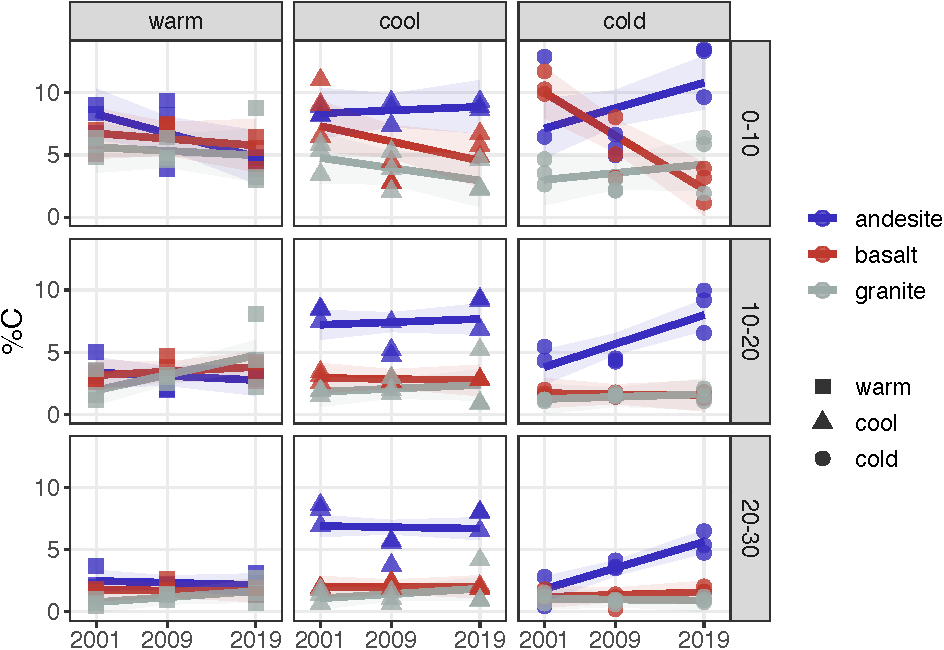
\includegraphics{sra-blk-inc-SI_files/figure-latex/plot-C-timeseries-1} 

}

\caption{Changes in soil C concentration, 2001-2019. Points show replicate profiles (n = 3); lines show marginal mean estimates of linear trends in soil C concentration with time; ribbons show 95\% CIs around trend estimates.}\label{fig:plot-C-timeseries}
\end{figure}

\clearpage

\hypertarget{respiration-fluxes}{%
\section{Respiration fluxes}\label{respiration-fluxes}}



\begin{figure}

{\centering 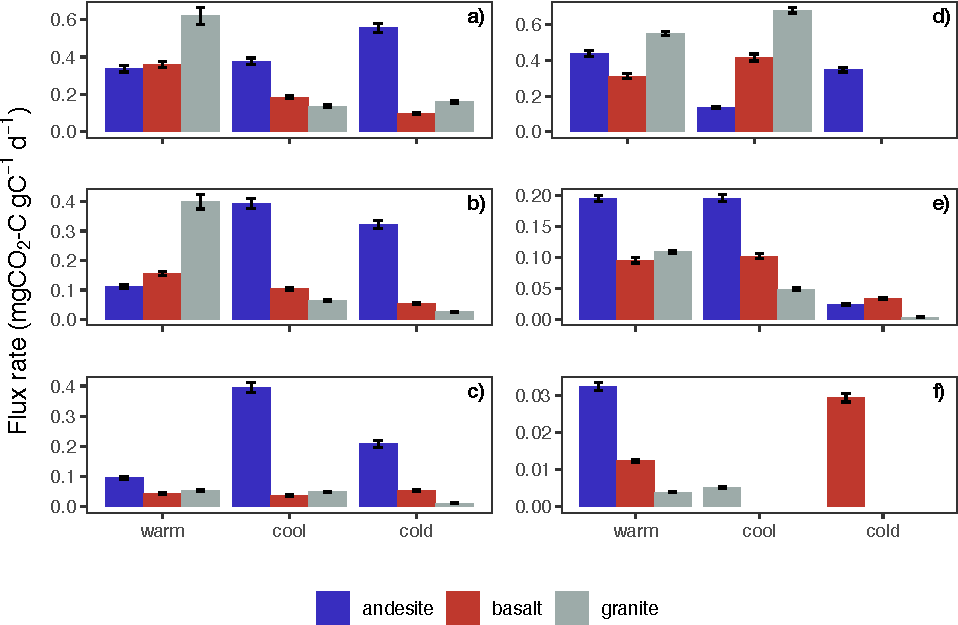
\includegraphics{sra-blk-inc-SI_files/figure-latex/plot-cmtv-flx-rates-1} 

}

\caption{Heterotrophic respiration rates from incubations of 2019 and 2001 samples. Panels a-c show 2019 data, and panels d-f show 2001 data. Panels in the top row (a, d) show the first depth increment for each year, middle row shows the second depth increment (b, e), and the bottom row shows the third depth increment (c, f). Bars show means for laboratory duplicates averaged over the whole incubation period; error bars ± 1 standard error of the mean. NB: Total CO\textsubscript{2} respired was controlled to be within 10,000 ppm (±1,000 ppm) for all samples; incubation duration varied between 4 and 40 days.}\label{fig:plot-cmtv-flx-rates}
\end{figure}

\clearpage

\hypertarget{radiocarbon-depth-profiles-2001-data}{%
\section{Radiocarbon depth profiles: 2001 data}\label{radiocarbon-depth-profiles-2001-data}}

Depth profiles of \(\Delta\)\textsuperscript{14}C\textsubscript{\emph{bulk}} were similar in 2001 (\textbf{Fig. \ref{fig:plot-d14c-pro-01}}) as to what we observed in 2019. We observed the most depleted \textsuperscript{14}C overall in the cool climate sites, where we also observed the clearest differences among parent materials. Parent material differences were least apparent for the cold climate sites, as we also observed in 2019. Within climate zones andesitic soils tended be most depleted and the granitic soils most enriched, with the basaltic parent material intermediate between the other two.



\begin{figure}

{\centering 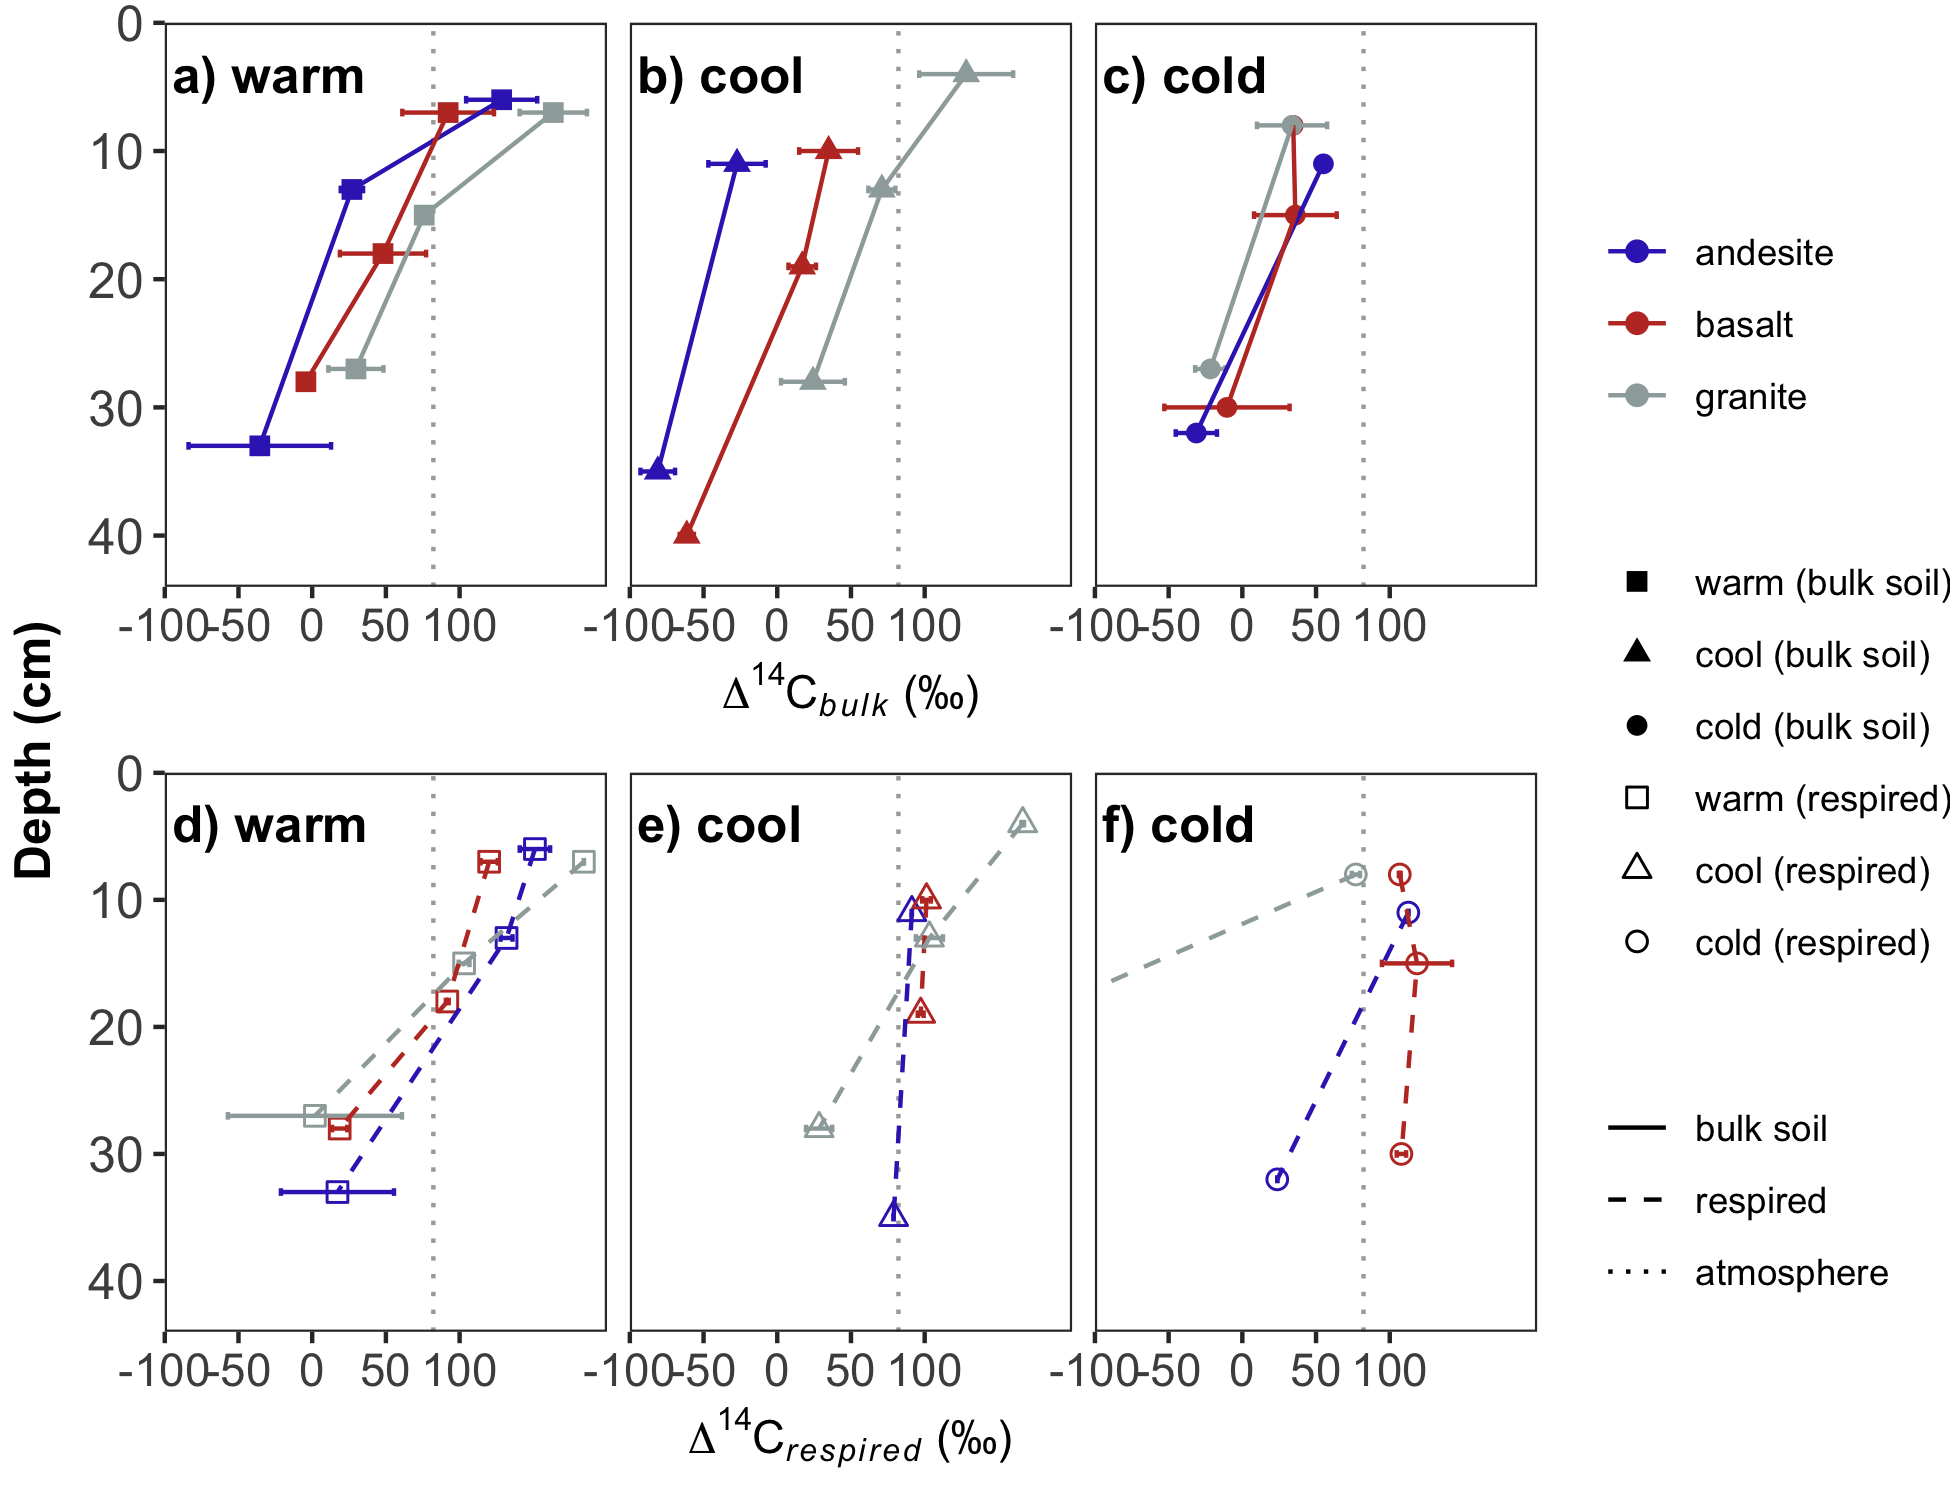
\includegraphics{sra-blk-inc-SI_files/figure-latex/plot-d14c-pro-01-1} 

}

\caption{Depth profiles of \(\Delta\)\textsuperscript{14}C\textsubscript{bulk} and \(\Delta\)\textsuperscript{14}C\textsubscript{respired} for 2001 data. Top panels show bulk data, bottom panels respired data. Dotted vertical lines show \(\Delta\)\textsuperscript{14}C of the atmosphere in the year of sampling. Points show the mean of three replicate profiles for bulk soil, and the mean of laboratory duplicates for respired CO\textsubscript{2}. Error bars show ±1 SD for bulk soils and the minimum and maximum for respired CO\textsubscript{2}. Respired CO\textsubscript{2} from the cold granite site (panel f) was extremely depleted in \(\Delta\)\textsuperscript{14}C and thus is excluded for display purposes.}\label{fig:plot-d14c-pro-01}
\end{figure}

\clearpage

\hypertarget{parent-material-and-climate-effects-on-bulk-and-respired-14c}{%
\section{\texorpdfstring{Parent material and climate effects on bulk and respired \textsuperscript{14}C}{Parent material and climate effects on bulk and respired 14C}}\label{parent-material-and-climate-effects-on-bulk-and-respired-14c}}

\hypertarget{contrasts}{%
\subsection{Contrasts}\label{contrasts}}





\begingroup\fontsize{10}{12}\selectfont

\begin{longtable}[t]{rllrrlrrl}
\caption{\label{tab:blk-inc-contrasts-10}Contrasts of bulk and respired \(\Delta\)\textsuperscript{14}C for parent material and climate factors, 0-0.1 m (all pairs). P value adjustment: Tukey method for comparing a family of 3 estimates.}\\
\toprule
\multicolumn{3}{c}{ } & \multicolumn{3}{c}{Bulk} & \multicolumn{3}{c}{Respired} \\
\cmidrule(l{3pt}r{3pt}){4-6} \cmidrule(l{3pt}r{3pt}){7-9}
Year & Group & Contrast & Est. & $SE$ & $p$ & Est. & $SE$ & $p$\\
\midrule
 &  & andesite - basalt & -62.0 & 18.8 & \textbf{0.011} &  &  & \\
\nopagebreak
 &  & andesite - granite & -124.5 & 18.8 & \textbf{< .001} &  &  & \\
\nopagebreak
 & \multirow[t]{-3}{*}{\raggedright\arraybackslash cool} & basalt - granite & -62.4 & 18.8 & \textbf{0.011} &  &  & \\
\nopagebreak
 &  & andesite - granite &  &  &  & 84.0 & 22.1 & \textbf{0.016}\\
\nopagebreak
 & \multirow[t]{-2}{*}{\raggedright\arraybackslash cold} & basalt - granite &  &  &  & 82.1 & 18.1 & \textbf{0.006}\\
\nopagebreak
 &  & warm - cool & 126.6 & 18.8 & \textbf{< .001} &  &  & \\
\nopagebreak
 & \multirow[t]{-2}{*}{\raggedright\arraybackslash andesite} & cool - cold & -82.1 & 21.0 & \textbf{0.003} &  &  & \\
\nopagebreak
 &  & warm - cool & 48.7 & 18.8 & \textbf{0.048} &  &  & \\
\nopagebreak
 & \multirow[t]{-2}{*}{\raggedright\arraybackslash basalt} & warm - cold & 66.1 & 18.8 & \textbf{0.007} &  &  & \\
\nopagebreak
 &  & warm - cold & 107.3 & 18.8 & \textbf{< .001} & 114.5 & 18.1 & \textbf{< .001}\\
\nopagebreak
\multirow[t]{-11}{*}{\raggedleft\arraybackslash 2001} & \multirow[t]{-2}{*}{\raggedright\arraybackslash granite} & cool - cold & 83.6 & 18.8 & \textbf{< .001} & 104.1 & 18.1 & \textbf{0.002}\\
\cmidrule{1-9}\pagebreak[0]
 &  & andesite - basalt & -56.5 & 16.3 & \textbf{0.007} &  &  & \\
\nopagebreak
 & \multirow[t]{-2}{*}{\raggedright\arraybackslash warm} & andesite - granite & -79.8 & 16.3 & \textbf{< .001} &  &  & \\
\nopagebreak
 & cool & basalt - granite &  &  &  & -43.6 & 18.0 & 0.089\\
\nopagebreak
 & andesite & cool - cold & -42.0 & 16.3 & \textbf{0.047} &  &  & \\
\nopagebreak
 & basalt & warm - cool & 52.3 & 16.3 & \textbf{0.013} &  &  & \\
\nopagebreak
 &  & warm - cool & 65.0 & 16.3 & \textbf{0.002} &  &  & \\
\nopagebreak
 &  & warm - cold & 58.5 & 16.3 & \textbf{0.006} & 47.1 & 18.0 & 0.066\\
\nopagebreak
\multirow[t]{-8}{*}{\raggedleft\arraybackslash 2019} & \multirow[t]{-3}{*}{\raggedright\arraybackslash granite} & cool - cold &  &  &  & 49.0 & 18.0 & 0.056\\
\bottomrule
\end{longtable}
\endgroup{}



\begingroup\fontsize{10}{12}\selectfont

\begin{longtable}[t]{rllrrlrrl}
\caption{\label{tab:blk-inc-contrasts-20}Contrasts of bulk and respired \(\Delta\)\textsuperscript{14}C for parent material and climate factors, 0.1-0.2 m (all pairs). P value adjustment: Tukey method for comparing a family of 3 estimates.}\\
\toprule
\multicolumn{3}{c}{ } & \multicolumn{3}{c}{Bulk} & \multicolumn{3}{c}{Respired} \\
\cmidrule(l{3pt}r{3pt}){4-6} \cmidrule(l{3pt}r{3pt}){7-9}
Year & Group & Contrast & Est. & $SE$ & $p$ & Est. & $SE$ & $p$\\
\midrule
 & warm & andesite - granite & -47.8 & 20.1 & 0.072 &  &  & \\
\nopagebreak
 &  & andesite - basalt & -72.2 & 20.1 & \textbf{0.006} &  &  & \\
\nopagebreak
 & \multirow[t]{-2}{*}{\raggedright\arraybackslash cool} & andesite - granite & -99.5 & 20.1 & \textbf{< .001} &  &  & \\
\nopagebreak
 &  & andesite - granite &  &  &  & 162.8 & 31.4 & \textbf{0.005}\\
\nopagebreak
 & \multirow[t]{-2}{*}{\raggedright\arraybackslash cold} & basalt - granite &  &  &  & 227.2 & 27.2 & \textbf{< .001}\\
\nopagebreak
 &  & warm - cool & 65.0 & 20.1 & \textbf{0.013} &  &  & \\
\nopagebreak
 & \multirow[t]{-2}{*}{\raggedright\arraybackslash andesite} & cool - cold & -57.2 & 22.5 & 0.052 &  &  & \\
\nopagebreak
 &  & warm - cold & 70.4 & 20.1 & \textbf{0.007} & 165.1 & 27.2 & \textbf{0.002}\\
\nopagebreak
\multirow[t]{-9}{*}{\raggedleft\arraybackslash 2001} & \multirow[t]{-2}{*}{\raggedright\arraybackslash granite} & cool - cold & 57.2 & 20.1 & \textbf{0.029} & 163.9 & 27.2 & \textbf{0.002}\\
\cmidrule{1-9}\pagebreak[0]
 &  & andesite - basalt & -62.6 & 20.1 & \textbf{0.016} &  &  & \\
\nopagebreak
 &  & andesite - granite & -124.9 & 20.1 & \textbf{< .001} & -52.4 & 13.7 & \textbf{0.013}\\
\nopagebreak
 & \multirow[t]{-3}{*}{\raggedright\arraybackslash warm} & basalt - granite & -62.3 & 20.1 & \textbf{0.016} & -35.2 & 13.7 & 0.078\\
\nopagebreak
 &  & andesite - basalt &  &  &  & 74.2 & 13.7 & \textbf{0.002}\\
\nopagebreak
 & \multirow[t]{-2}{*}{\raggedright\arraybackslash cool} & andesite - granite &  &  &  & 87.3 & 13.7 & \textbf{< .001}\\
\nopagebreak
 &  & andesite - granite &  &  &  & 62.2 & 16.8 & \textbf{0.015}\\
\nopagebreak
 & \multirow[t]{-2}{*}{\raggedright\arraybackslash cold} & basalt - granite &  &  &  & 70.8 & 16.8 & \textbf{0.007}\\
\nopagebreak
 &  & warm - cool & 74.8 & 20.1 & \textbf{0.004} & 63.0 & 13.7 & \textbf{0.004}\\
\nopagebreak
 & \multirow[t]{-2}{*}{\raggedright\arraybackslash basalt} & cool - cold & -63.5 & 20.1 & \textbf{0.014} & -54.2 & 13.7 & \textbf{0.011}\\
\nopagebreak
 &  & warm - cool & 118.2 & 20.1 & \textbf{< .001} & 111.3 & 13.7 & \textbf{< .001}\\
\nopagebreak
\multirow[t]{-11}{*}{\raggedleft\arraybackslash 2019} & \multirow[t]{-2}{*}{\raggedright\arraybackslash granite} & warm - cold & 105.3 & 20.1 & \textbf{< .001} & 114.7 & 16.8 & \textbf{< .001}\\
\bottomrule
\end{longtable}
\endgroup{}



\begingroup\fontsize{10}{12}\selectfont

\begin{longtable}[t]{rllrrlrrl}
\caption{\label{tab:blk-inc-contrasts-30}Contrasts of bulk and respired \(\Delta\)\textsuperscript{14}C for parent material and climate factors, 0.2-0.3 m (all pairs). P value adjustment: Tukey method for comparing a family of 3 estimates.}\\
\toprule
\multicolumn{3}{c}{ } & \multicolumn{3}{c}{Bulk} & \multicolumn{3}{c}{Respired} \\
\cmidrule(l{3pt}r{3pt}){4-6} \cmidrule(l{3pt}r{3pt}){7-9}
Year & Group & Contrast & Est. & $SE$ & $p$ & Est. & $SE$ & $p$\\
\midrule
 & warm & andesite - granite & -70.2 & 21.0 & \textbf{0.01} &  &  & \\
\nopagebreak
 &  & andesite - granite & -106.5 & 21.0 & \textbf{< .001} &  &  & \\
\nopagebreak
 & \multirow[t]{-2}{*}{\raggedright\arraybackslash cool} & basalt - granite & -62.9 & 21.0 & \textbf{0.021} &  &  & \\
\nopagebreak
\multirow[t]{-4}{*}{\raggedleft\arraybackslash 2001} & granite & warm - cold & 51.8 & 21.0 & 0.061 &  &  & \\
\cmidrule{1-9}\pagebreak[0]
 &  & andesite - granite & -51.9 & 19.6 & \textbf{0.042} &  &  & \\
\nopagebreak
 & \multirow[t]{-2}{*}{\raggedright\arraybackslash warm} & basalt - granite & -51.3 & 19.6 & \textbf{0.044} &  &  & \\
\nopagebreak
 &  & andesite - basalt &  &  &  & 93.9 & 20.6 & \textbf{0.005}\\
\nopagebreak
 & \multirow[t]{-2}{*}{\raggedright\arraybackslash cool} & basalt - granite & -53.5 & 19.6 & \textbf{0.035} & -61.0 & 20.6 & \textbf{0.043}\\
\nopagebreak
 & cold & andesite - basalt & -46.3 & 19.6 & 0.073 &  &  & \\
\nopagebreak
 & andesite & warm - cool & 57.6 & 19.6 & \textbf{0.023} &  &  & \\
\nopagebreak
 &  & warm - cool & 75.7 & 19.6 & \textbf{0.003} & 64.7 & 20.6 & \textbf{0.033}\\
\nopagebreak
 & \multirow[t]{-2}{*}{\raggedright\arraybackslash basalt} & cool - cold & -106.5 & 19.6 & \textbf{< .001} & -86.8 & 25.3 & \textbf{0.022}\\
\nopagebreak
 &  & warm - cool & 73.5 & 19.6 & \textbf{0.004} &  &  & \\
\nopagebreak
\multirow[t]{-10}{*}{\raggedleft\arraybackslash 2019} & \multirow[t]{-2}{*}{\raggedright\arraybackslash granite} & warm - cold & 51.5 & 19.6 & \textbf{0.043} & 57.8 & 20.6 & 0.054\\
\bottomrule
\end{longtable}
\endgroup{}

\clearpage

\hypertarget{temporal-trends-contrasts}{%
\subsection{Temporal trends \& contrasts}\label{temporal-trends-contrasts}}

Please see the main text for discussion of the temporal trends in both \(\Delta\)\textsuperscript{14}C\textsubscript{\emph{bulk}} and \(\Delta\)\textsuperscript{14}C\textsubscript{\emph{bulk}}. See SI tables \textbf{\ref{tab:blk-trend-stats}} and \textbf{\ref{tab:inc-trend-stats}} for statistics.



\begingroup\fontsize{10}{12}\selectfont

\begin{longtable}[t]{lllrlrlr}
\caption{\label{tab:blk-trend-stats}Change in \(\Delta\)\textsuperscript{14}C\textsubscript{\emph{bulk}}, 2001-2019. Degrees of freedom = 44; confidence level used = 0.95.}\\
\toprule
\multicolumn{2}{c}{ } & \multicolumn{2}{c}{0-10cm} & \multicolumn{2}{c}{10-20cm} & \multicolumn{2}{c}{20-30cm} \\
\cmidrule(l{3pt}r{3pt}){3-4} \cmidrule(l{3pt}r{3pt}){5-6} \cmidrule(l{3pt}r{3pt}){7-8}
Climate & Parent material & Trend & $SE$ & Trend & $SE$ & Trend & $SE$\\
\midrule
\endfirsthead
\caption[]{\label{tab:blk-trend-stats}Change in \(\Delta\)\textsuperscript{14}C\textsubscript{\emph{bulk}}, 2001-2019. Degrees of freedom = 44; confidence level used = 0.95. \textit{(continued)}}\\
\toprule
\multicolumn{2}{c}{ } & \multicolumn{2}{c}{0-10cm} & \multicolumn{2}{c}{10-20cm} & \multicolumn{2}{c}{20-30cm} \\
\cmidrule(l{3pt}r{3pt}){3-4} \cmidrule(l{3pt}r{3pt}){5-6} \cmidrule(l{3pt}r{3pt}){7-8}
Climate & Parent material & Trend & $SE$ & Trend & $SE$ & Trend & $SE$\\
\midrule
\endhead

\endfoot
\bottomrule
\endlastfoot
 & andesite & \textbf{-5.8} & 1.0 & -1.9 & 1.3 & 1.1 & 1.3\\
\nopagebreak
 & basalt & -1.8 & 1.0 & -0.1 & 1.3 & -1.1 & 1.3\\
\nopagebreak
\multirow[t]{-3}{*}{\raggedright\arraybackslash warm} & granite & \textbf{-2.5} & 1.0 & 2.4 & 1.3 & 0.2 & 1.3\\
\cmidrule{1-8}\pagebreak[0]
 & andesite & 0.1 & 1.0 & 0.4 & 1.3 & 0.3 & 1.3\\
\nopagebreak
 & basalt & -2.1 & 1.0 & \textbf{-3.2} & 1.3 & \textbf{-3.3} & 1.3\\
\nopagebreak
\multirow[t]{-3}{*}{\raggedright\arraybackslash cool} & granite & \textbf{-4.9} & 1.0 & \textbf{-3.5} & 1.3 & \textbf{-3.6} & 1.3\\
\cmidrule{1-8}\pagebreak[0]
 & andesite & -2.2 & 1.1 & -0.9 & 1.4 & 0.4 & 1.5\\
\nopagebreak
 & basalt & 0.9 & 1.0 & 0 & 1.3 & 1.4 & 1.3\\
\nopagebreak
\multirow[t]{-3}{*}{\raggedright\arraybackslash cold} & granite & 0.1 & 1.0 & 0.3 & 1.3 & 0.1 & 1.3\\*
\end{longtable}
\endgroup{}



\begingroup\fontsize{10}{12}\selectfont

\begin{longtable}[t]{lllrlrlr}
\caption{\label{tab:inc-trend-stats}Change in \(\Delta\)\textsuperscript{14}C\textsubscript{\emph{respired}}, 2001-2019. Degrees of freedom = 44; confidence level used = 0.95.}\\
\toprule
\multicolumn{2}{c}{ } & \multicolumn{2}{c}{0-10cm} & \multicolumn{2}{c}{10-20cm} & \multicolumn{2}{c}{20-30cm} \\
\cmidrule(l{3pt}r{3pt}){3-4} \cmidrule(l{3pt}r{3pt}){5-6} \cmidrule(l{3pt}r{3pt}){7-8}
Climate & Parent material & Trend & $SE$ & Trend & $SE$ & Trend & $SE$\\
\midrule
\endfirsthead
\caption[]{\label{tab:inc-trend-stats}Change in \(\Delta\)\textsuperscript{14}C\textsubscript{\emph{respired}}, 2001-2019. Degrees of freedom = 44; confidence level used = 0.95. \textit{(continued)}}\\
\toprule
\multicolumn{2}{c}{ } & \multicolumn{2}{c}{0-10cm} & \multicolumn{2}{c}{10-20cm} & \multicolumn{2}{c}{20-30cm} \\
\cmidrule(l{3pt}r{3pt}){3-4} \cmidrule(l{3pt}r{3pt}){5-6} \cmidrule(l{3pt}r{3pt}){7-8}
Climate & Parent material & Trend & $SE$ & Trend & $SE$ & Trend & $SE$\\
\midrule
\endhead

\endfoot
\bottomrule
\endlastfoot
 & andesite & \textbf{-6.2} & 1.0 & -2.1 & 1.0 & 1.4 & 2.0\\
\nopagebreak
 & basalt & \textbf{-2.3} & 1.0 & -0.9 & 1.0 & 0.4 & 2.0\\
\nopagebreak
\multirow[t]{-3}{*}{\raggedright\arraybackslash warm} & granite & \textbf{-3.7} & 1.0 & 2 & 1.0 & 3.2 & 2.0\\
\cmidrule{1-8}\pagebreak[0]
 & andesite & -1.4 & 1.2 & -1 & 1.2 & -1.5 & 2.5\\
\nopagebreak
 & basalt & \textbf{-3.7} & 1.0 & \textbf{-5.9} & 1.0 & NA & \\
\nopagebreak
\multirow[t]{-3}{*}{\raggedright\arraybackslash cool} & granite & \textbf{-3} & 1.0 & \textbf{-4.1} & 1.0 & 0 & 2.0\\
\cmidrule{1-8}\pagebreak[0]
 & andesite & \textbf{-2.9} & 1.2 & -0.8 & 1.2 & 1.4 & 2.5\\
\nopagebreak
 & basalt & \textbf{-3.9} & 1.0 & \textbf{-3.9} & 1.0 & -3.5 & 2.5\\
\nopagebreak
\multirow[t]{-3}{*}{\raggedright\arraybackslash cold} & granite & 0.1 & 1.0 & \textbf{4.8} & 1.4 & NA & \\*
\end{longtable}
\endgroup{}

We saw more significant contrasts in the change over time in \(\Delta\)\textsuperscript{14}C\textsubscript{\emph{respired}} than we did for \(\Delta\)\textsuperscript{14}C\textsubscript{\emph{bulk}} (\textbf{Table \ref{tab:blk-inc-trend-contrasts}}). When considered within climate zones, trends for the basaltic and granitic soils were more similar to one another overall than were either to the andesitic soils. We observed parent material trend contrasts more commonly in the cool and cold climate sites than in the warm sites; however we only observed significant trend contrasts for the cold climate sites in the \(\Delta\)\textsuperscript{14}C\textsubscript{\emph{respired}} data, and not for \(\Delta\)\textsuperscript{14}C\textsubscript{\emph{bulk}}. When considered within parent materials, we saw more siginificant trend contrasts for the granitic and basaltic soils than for the andesitic soils (\textbf{Table \ref{tab:blk-inc-trend-contrasts}}).



\begingroup\fontsize{10}{12}\selectfont

\begin{longtable}[t]{lllrrlrrl}
\caption{\label{tab:blk-inc-trend-contrasts}Contrasts for bulk and respired \(\Delta\)\textsuperscript{14}C by year and depth. P value adjustment: Tukey method for comparing a family of 3 estimates.}\\
\toprule
\multicolumn{3}{c}{ } & \multicolumn{3}{c}{Bulk} & \multicolumn{3}{c}{Respired} \\
\cmidrule(l{3pt}r{3pt}){4-6} \cmidrule(l{3pt}r{3pt}){7-9}
Depth & Group & Contrast & Est. & $SE$ & $p$ & Est. & $SE$ & $p$\\
\midrule
\endfirsthead
\caption[]{\label{tab:blk-inc-trend-contrasts}Contrasts for bulk and respired \(\Delta\)\textsuperscript{14}C by year and depth. P value adjustment: Tukey method for comparing a family of 3 estimates. \textit{(continued)}}\\
\toprule
\multicolumn{3}{c}{ } & \multicolumn{3}{c}{Bulk} & \multicolumn{3}{c}{Respired} \\
\cmidrule(l{3pt}r{3pt}){4-6} \cmidrule(l{3pt}r{3pt}){7-9}
Depth & Group & Contrast & Est. & $SE$ & $p$ & Est. & $SE$ & $p$\\
\midrule
\endhead

\endfoot
\bottomrule
\endlastfoot
 & warm & andesite - basalt & -4.0 & 1.4 & \textbf{0.021} & -3.9 & 1.4 & \textbf{0.036}\\
\nopagebreak
 & warm & andesite - granite & -3.3 & 1.4 & 0.068 &  &  & \\
\nopagebreak
 & cool & andesite - granite & 5.0 & 1.4 & \textbf{0.004} &  &  & \\
\nopagebreak
 & cold & basalt - granite &  &  &  & -4.0 & 1.4 & \textbf{0.031}\\
\nopagebreak
 & andesite & warm - cool & -5.9 & 1.4 & \textbf{< .001} & -4.8 & 1.6 & \textbf{0.021}\\
\nopagebreak
 & andesite & warm - cold & -3.6 & 1.5 & 0.06 &  &  & \\
\nopagebreak
 & granite & warm - cold &  &  &  & -3.7 & 1.4 & \textbf{0.045}\\
\nopagebreak
\multirow[t]{-8}{*}{\raggedright\arraybackslash 0-10cm} & granite & cool - cold & -5.0 & 1.4 & \textbf{0.004} &  &  & \\
\cmidrule{1-9}\pagebreak[0]
 & warm & andesite - granite & -4.3 & 1.8 & 0.051 & -4.1 & 1.4 & \textbf{0.03}\\
\nopagebreak
 & cool & andesite - basalt &  &  &  & 4.9 & 1.6 & \textbf{0.019}\\
\nopagebreak
 & cool & andesite - granite & 4.0 & 1.8 & 0.08 &  &  & \\
\nopagebreak
 & cold & andesite - granite &  &  &  & -5.6 & 1.9 & \textbf{0.024}\\
\nopagebreak
 & cold & basalt - granite &  &  &  & -8.7 & 1.7 & \textbf{< .001}\\
\nopagebreak
 & basalt & warm - cool &  &  &  & 5.0 & 1.4 & \textbf{0.008}\\
\nopagebreak
 & granite & warm - cool & 5.9 & 1.8 & \textbf{0.005} & 6.1 & 1.4 & \textbf{0.002}\\
\nopagebreak
\multirow[t]{-8}{*}{\raggedright\arraybackslash 10-20cm} & granite & cool - cold & -3.8 & 1.8 & 0.094 & -8.9 & 1.7 & \textbf{< .001}\\
\cmidrule{1-9}\pagebreak[0]
20-30cm & basalt & cool - cold & -4.7 & 1.9 & \textbf{0.04} &  &  & \\*
\end{longtable}
\endgroup{}

\clearpage

\hypertarget{mineral-assemblages}{%
\section{Mineral assemblages}\label{mineral-assemblages}}

We simplified the data in the main text to consider the relationship between \(\Delta\)\textsuperscript{14}C and either poorly crystalline metal oxides or crystalline metal oxides. We present here the individual regression plots for \(\Delta\)\textsuperscript{14}C\textsubscript{\emph{bulk}} (\textbf{Fig. \ref{fig:min-blk30-plot}}) and \(\Delta\)\textsuperscript{14}C\textsubscript{\emph{respired}} (\textbf{Fig. \ref{fig:min-inc30-plot}}).

We also present here the results of the individual regression analyses for \(\Delta\)\textsuperscript{14}C\textsubscript{\emph{bulk}} (\textbf{Fig. \ref{fig:min-all-blk-plot}}), \(\Delta\)\textsuperscript{14}C\textsubscript{\emph{respired}} (\textbf{Fig. \ref{fig:min-all-inc-plot}}), and \(\Delta\)\textsuperscript{14}C\textsubscript{\emph{respired-bulk}} vs.~Al selectively dissolved with ammonium oxalate (Al\textsubscript{o}) or sodium pyrophosphate (Al\textsubscript{p}), and Fe selectively dissolved with ammonium oxalate (Fe\textsubscript{o}), or dithionite citrate (Fe\textsubscript{d}) \textbf{Fig. \ref{fig:min-all-inc-blk-plot}}. The relationships between Al\textsubscript{o}, Al\textsubscript{p}, and Fe\textsubscript{o} and \(\Delta\)\textsuperscript{14}C\textsubscript{\emph{respired-bulk}} in the models derived from Eq. (4) (main text) were all highly significant (\emph{p} \textless{} 0.001). P-values for the metal oxide concentration coefficients in the \(\Delta\)\textsuperscript{14}C\textsubscript{\emph{respired-bulk}} and \(\Delta\)\textsuperscript{14}C\textsubscript{\emph{bulk}} models were highly significant (\textless{} 0.001 at \(\alpha\) = 0.1) for Al\textsubscript{o}, Al\textsubscript{p}, and Fe\textsubscript{o}. The coefficient for Al\textsubscript{o} in \(\Delta\)\textsuperscript{14}C\textsubscript{\emph{respired}} model also had a p-value of \textless{} 0.001, but while still significant, p-values were larger for Al\textsubscript{p} and Fe\textsubscript{o} in the \(\Delta\)\textsuperscript{14}C\textsubscript{\emph{respired}} models: 0.028, 0.086, respectively.
In contrast, the concentration of Fe\textsubscript{d} was not significant in any of the models.



\begin{figure}

{\centering 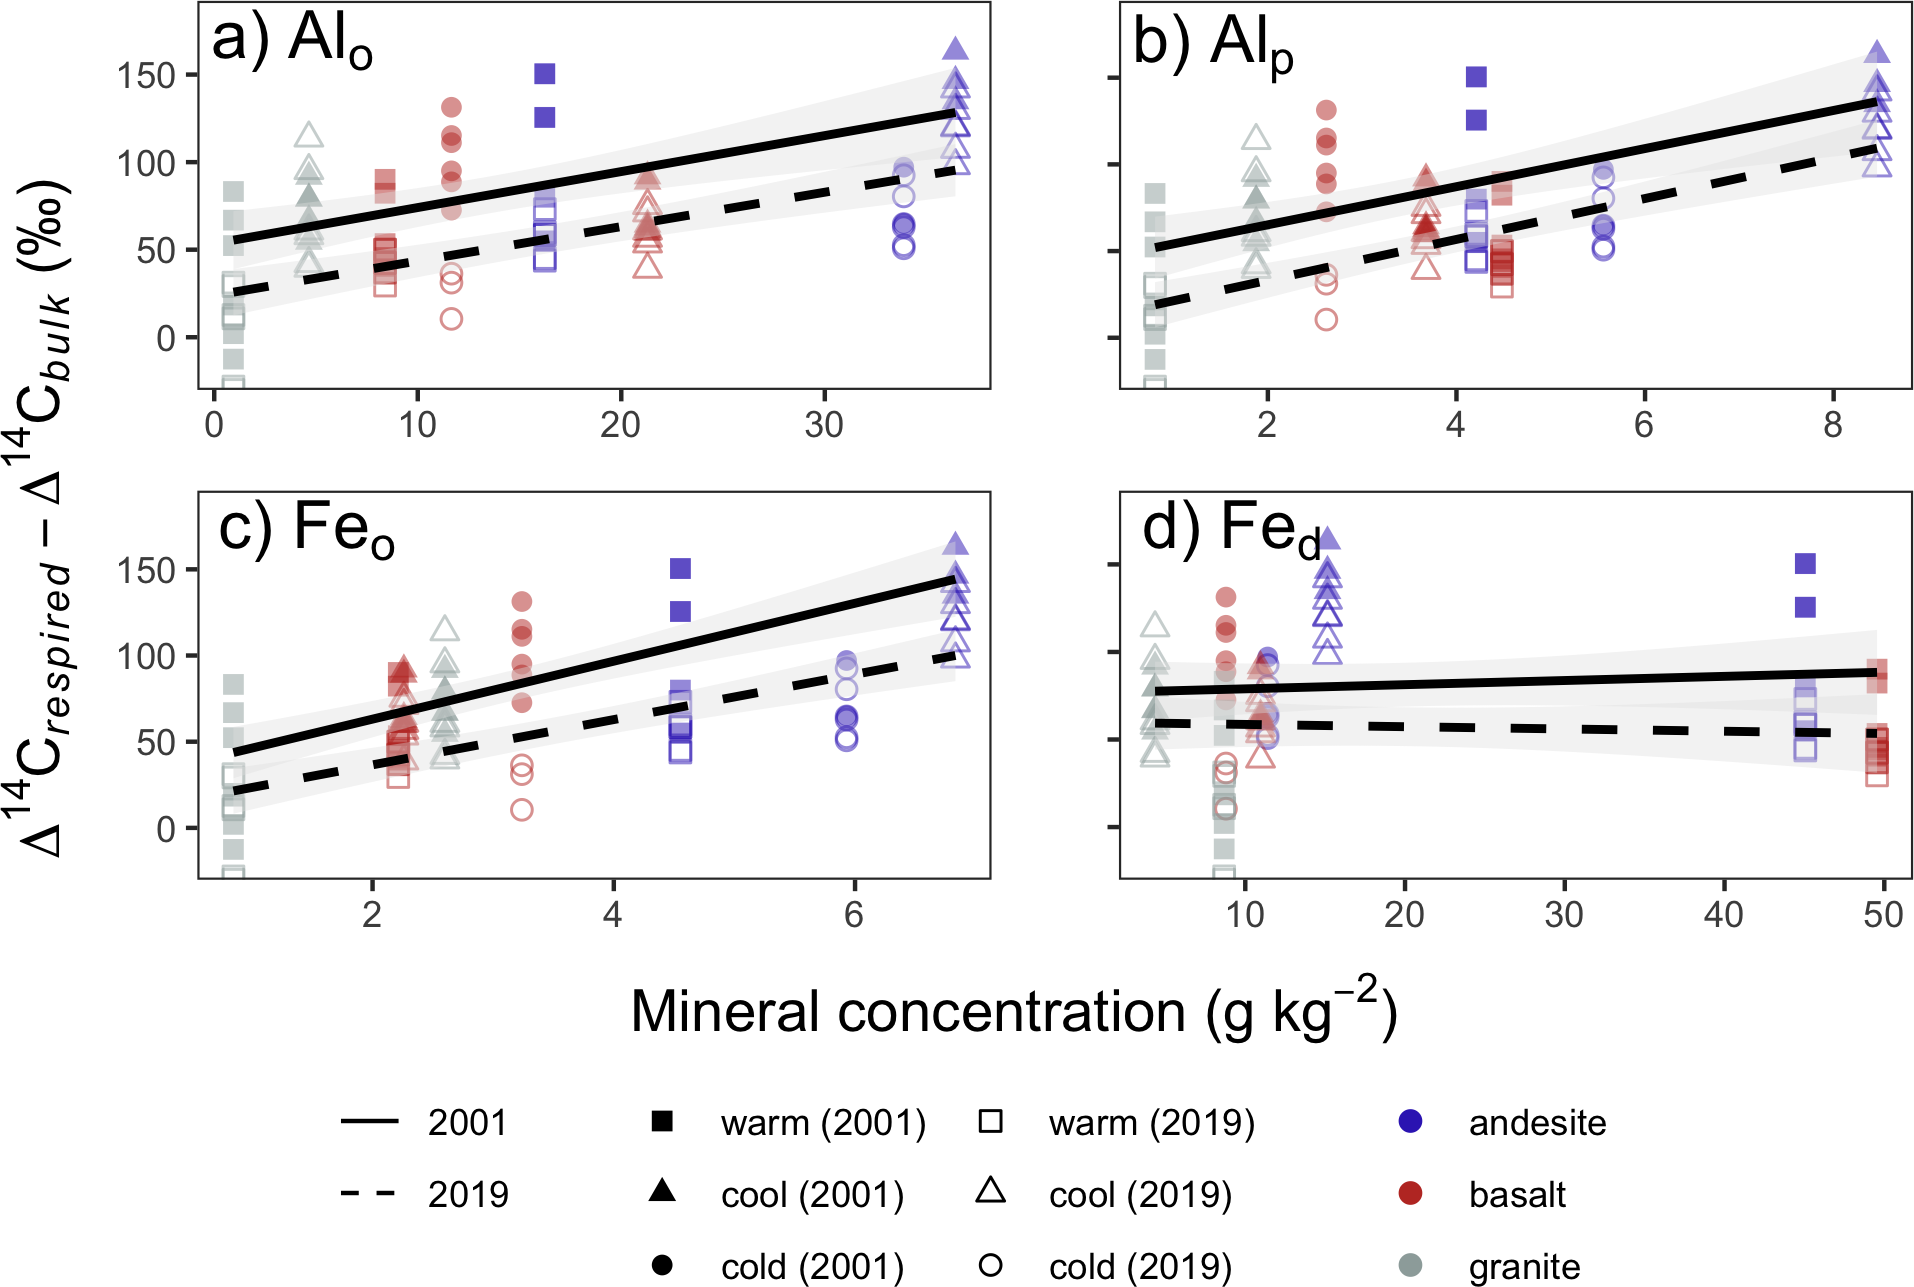
\includegraphics{sra-blk-inc-SI_files/figure-latex/min-all-inc-blk-plot-1} 

}

\caption{Relationship of selectively dissolved iron and alumnimum to the difference between \(\Delta\)\textsuperscript{14}C\textsubscript{\emph{respired}} and \(\Delta\)\textsuperscript{14}C\textsubscript{\emph{bulk}} (\(\Delta\)\textsuperscript{14}C\textsubscript{\emph{respired-bulk}}). (a) Oxalate-extractable aluminum (Al\textsubscript{o}), (b) Pyrophosphate-extractable aluminum (Al\textsubscript{p}), (c) Oxalate-extractable iron (Fe\textsubscript{o}), (d) Dithionite extractable iron (Fe\textsubscript{d}). Points show mass-weighted mineral concentrations and carbon-weighted values of \(\Delta\)\textsuperscript{14}C\textsubscript{\emph{respired-bulk}} for 0-30cm profiles. Lines show linear model fits from Eq. (5) (main text).}\label{fig:min-all-inc-blk-plot}
\end{figure}



\begin{figure}

{\centering 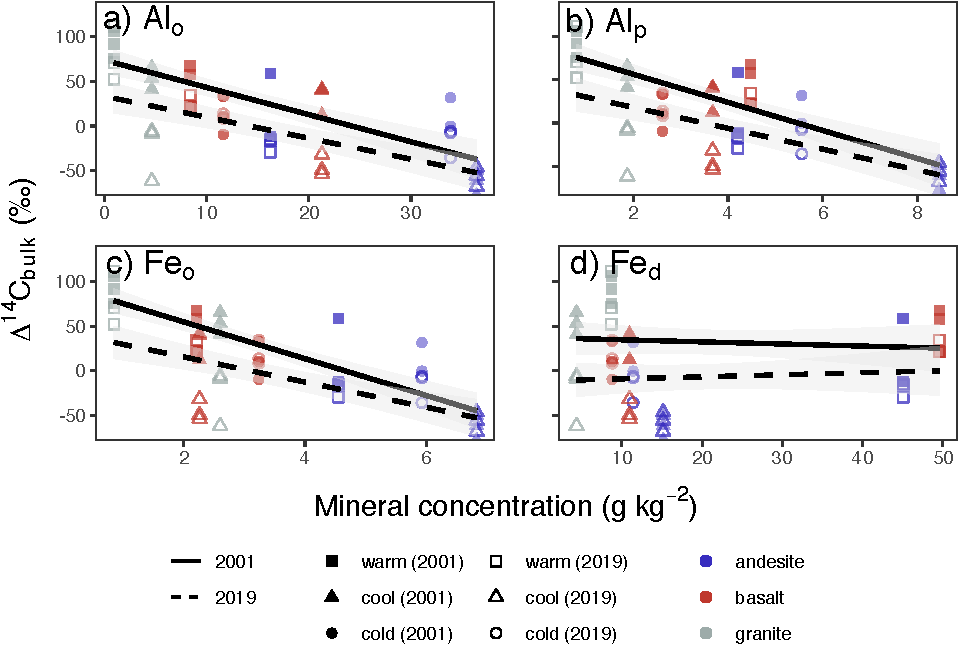
\includegraphics{sra-blk-inc-SI_files/figure-latex/min-all-blk-plot-1} 

}

\caption{Relationship of selectively dissolved iron and alumnimum to \(\Delta\)\textsuperscript{14}C\textsubscript{\emph{bulk}}. (a) Oxalate-extractable aluminum (Al\textsubscript{o}), (b) Pyrophosphate-extractable aluminum (Al\textsubscript{p}), (c) Oxalate-extractable iron (Fe\textsubscript{o}), (d) Dithionite extractable iron (Fe\textsubscript{d}). Points show mass-weighted mineral concentrations and carbon-weighted values of \(\Delta\)\textsuperscript{14}C\textsubscript{\emph{bulk}} for 0-30cm profiles. Lines show linear model fits from Eq. (5) (main text).}\label{fig:min-all-blk-plot}
\end{figure}



\begin{figure}

{\centering 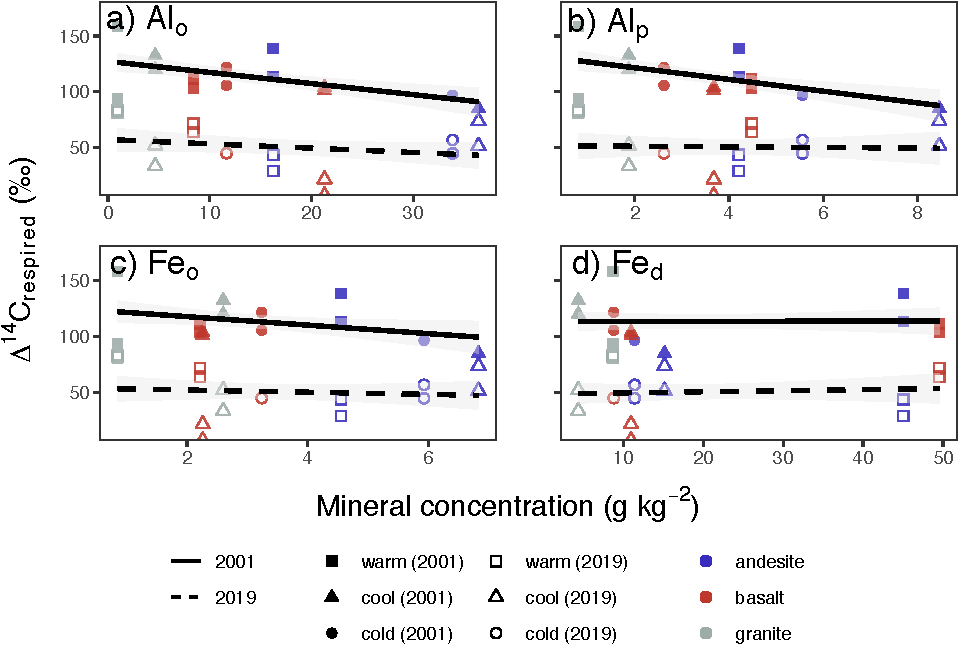
\includegraphics{sra-blk-inc-SI_files/figure-latex/min-all-inc-plot-1} 

}

\caption{Relationship of selectively dissolved iron and alumnimum to \(\Delta\)\textsuperscript{14}C\textsubscript{\emph{respired}}. (a) Oxalate-extractable aluminum (Al\textsubscript{o}), (b) Pyrophosphate-extractable aluminum (Al\textsubscript{p}), (c) Oxalate-extractable iron (Fe\textsubscript{o}), (d) Dithionite extractable iron (Fe\textsubscript{d}). Points show mass-weighted mineral concentrations and carbon-weighted values of \(\Delta\)\textsuperscript{14}C\textsubscript{\emph{respired}} for 0-30cm profiles. Lines show linear model fits from Eq. (5) (main text).}\label{fig:min-all-inc-plot}
\end{figure}



\begin{figure}

{\centering 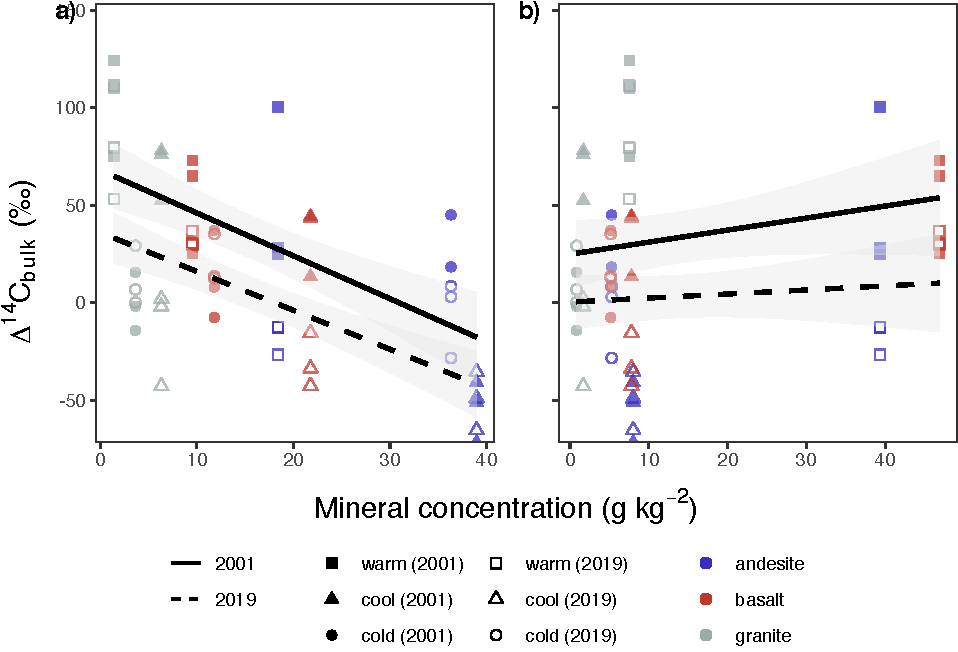
\includegraphics{sra-blk-inc-SI_files/figure-latex/min-blk30-plot-1} 

}

\caption{Relationship of poorly crystalline and crystalline minerals to \(\Delta\)\textsuperscript{14}C\textsubscript{\emph{bulk}}. (a) Poorly crystalline mineral content (oxalate-extractable aluminum + 1/2 oxalate-extractable iron), (b) Crystalline mineral content (dithionite-extractable iron - oxalate-extractable iron). Points show mass-weighted mineral concentrations and carbon-weighted values of \(\Delta\)\textsuperscript{14}C\textsubscript{\emph{bulk}} for 0-30cm profiles. Lines show linear model fits from Eq. (5) (main text).}\label{fig:min-blk30-plot}
\end{figure}



\begin{figure}

{\centering 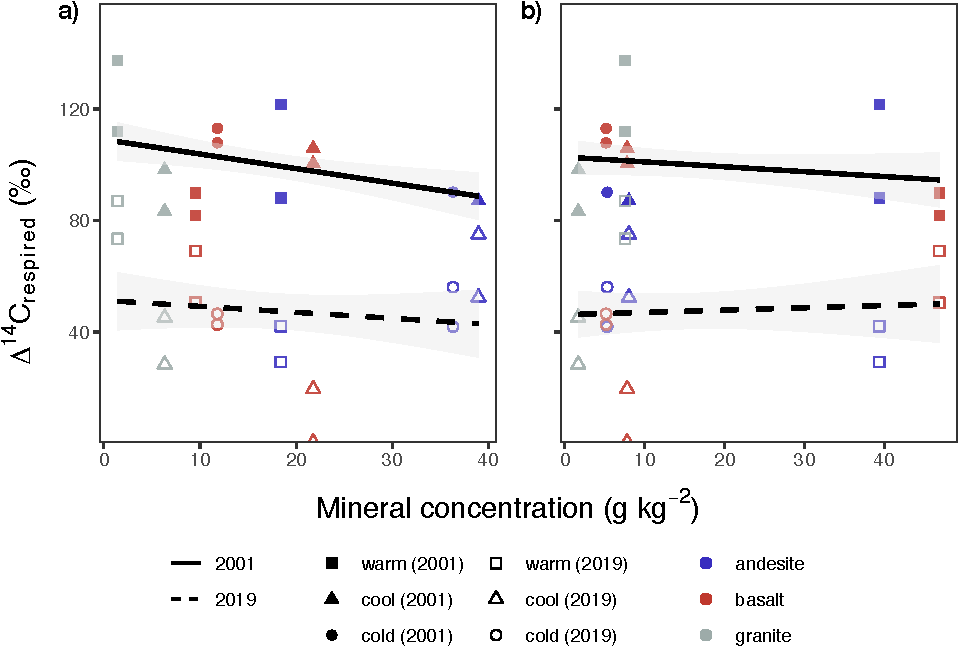
\includegraphics{sra-blk-inc-SI_files/figure-latex/min-inc30-plot-1} 

}

\caption{Relationship of poorly crystalline and crystalline minerals to \(\Delta\)\textsuperscript{14}C\textsubscript{\emph{respired}}. (a) Poorly crystalline mineral content (oxalate-extractable aluminum + 1/2 oxalate-extractable iron), (b) Crystalline mineral content (dithionite-extractable iron - oxalate-extractable iron). Points show mass-weighted mineral concentrations and carbon-weighted values of \(\Delta\)\textsuperscript{14}C\textsubscript{\emph{respired}} for 0-30cm profiles. Lines show linear model fits from Eq. (5) (main text).}\label{fig:min-inc30-plot}
\end{figure}


\clearpage
\renewcommand{\listfigurename}{Figure captions}

\clearpage
\renewcommand{\listtablename}{Table captions}


\end{document}
